\clearpage{\pagestyle{empty}\cleardoublepage}

\chapter{Monte Carlo simulation}\label{chap:mc}

In science, little should be left to chance. Still, randomness
over a huge number of trials leads to insights of something we could
consider as ``real''. This is particularly useful when dealing with 
complex environments that can be described with a mathematical model
in order to know what to expect from the actual data.
Monte Carlo methods can describe hadron-hadron collisions,
using pseudorandom numbers to simulate event-by-event fluctuations, and
hence help us e.g. understand the detector response and develop analysis
strategies by predicting the sensitivity to the physics under study.

In this chapter, we will first go through a very brief overview of some concepts of the 
Quantum Chromodynamics theory useful to understand the evolution of a pp collision
event (Section~\ref{sec:MCphenomenology}). Thanks to perturbation theory we can predict hard 
scattering cross sections, which is what is done as the first step of the Monte Carlo 
simulation chain, described in Section~\ref{sec:matrixelement}.
Despite the theoretical ability to compute fixed order calculations for hard scattering cross sections,
%this does not allow us to describe a specific final state, plus we still lack the possibility to 
we still lack the possibility to describe QCD at low energy and, hence, hadron final states formation. 
{\it Shower algorithms} can associate to a hard event an arbitrary number of partons to constitute
a final state with quarks and gluons (see Section~\ref{sec:partonshower}). 
The {\it hadronization} of this yet unphysical final state is
performed by means of phenomenological models of hadron formation, introduced in Section~\ref{sec:hadronization}. 
The last ingredient for a complete picture is the treatment of
the remnants of the incoming protons the hard interacting partons
came from. For this we rely on the so-called ``underlying event model'', discussed in 
Section~\ref{sec:underlyingevent}.

Finally, the products from the generated event are passed through a simulation of the ATLAS
detector geometry and response, and digitized to give an output identical to 
that of the real detector (Section~\ref{sec:MCdetector}).
At this point physics objects are reconstructed in the same way for Monte Carlo
and real data, as discussed in Chapter~\ref{chap:objects}.
 

\section{Phenomenology of pp collisions}\label{sec:MCphenomenology}

The most challenging aspect of the simulation of
hadron collider physics is the 
%Of the interactions making up the processes, for Monte Carlo simulating
%hadron colliders physics the most challenging part is related to the
description of Quantum Chromodynamics (QCD) phenomenology. Indeed,
despite its theorethical framework being successful and verified, calculations
are difficult and often need approximations.

\subsection{Proton structure}

The proton is a bound state of three {\it valence} quarks with each carrying
a fraction $x$ of the proton momentum. Such momentum fraction is described
by parton distribution functions (PDFs) $f_i(x,\mu)$ which need to be measured 
experimentally at a certain transferred momentum $\mu$. 
It is observed that the valence quarks only carry about half of the proton total
momentum, the rest being carried by virtual gluons continuatively exchanged 
by the quarks. These gluons in turn produce virtual $q\bar{q}$ pairs called
{\it sea} quarks.
The probability for a parton $i$
to carry a momentum fraction between $x$ and $x+dx$ is $f_i(x,\mu)dx$ and the following
condition holds:
\begin{equation}
\int_0^1 x \sum  \limits_i f_i(x) dx = 1,
\end{equation}
where the sum goes over all the parton flavors considered (typically $u,d,s,c,b,g$).

PDFs are measured in deep inelastic scattering experiments and at hadron colliders and 
are universal, not depending on the particular process used.
Various parametrizations are available and the most widely used come from the
CTEQ and MRST/MSTW collaborations~\cite{mrstcoll,mrst,mstwcoll,mstw}\footnote{See for more information
the Les Houches Accord PDFs (LHAPDF): \url{http://lhapdf.hepforge.org/}.}.
%and the collaborations pages: \url{http://www.phys.psu.edu/cteq}, 
%\url{http://mstwpdf.hepforge.org/}.}
The PDFs of valence quarks, gluon and sea quarks 
from the MSTW group are shown in Figure~\ref{fig:PDFs} as a function of the 
momentum fraction for two values of transferred momentum Q$^2$
at which the proton is probed.

\begin{figure}[tbph]
\begin{center}
\subfigure{
  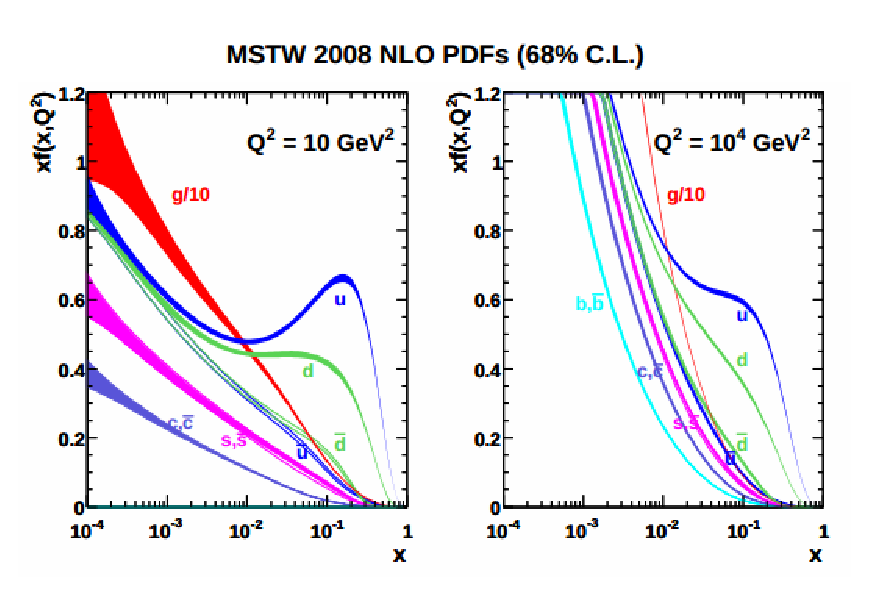
\includegraphics[width=0.75\textwidth]{montecarlo/figures/pdfs2.eps}
}
\caption{Proton PDF functions at transfer momentum
 Q$^2$=10$~$GeV$^2$ (Q$^2$=10000$~$GeV$^2$) on the left (right)~\cite{Martin:2009iq}.\label{fig:PDFs}}
\end{center}
\end{figure}



\subsection{Factorization theorem}\label{sec:factorization}

To treat infinities arising from divergent contributions in loop diagrams like
the ones of Figure~\ref{fig:feyndLOOP},
an arbitrary renormalization scale $\mu_R$ is to be introduced. As a consequence
from requiring that the physical observables be independent from the choice of $\mu_R$,
the strong coupling constant $\alphas$ does depend on the energy scale at which the 
coupling is observed and is, at the leading order:

\begin{equation}\label{eq:alphas}
\alphas(\mu^2) = \dfrac{\alphas(\mu_R^2)}{1 + (11 - \frac{2}{3}n_f)\frac{\alphas(\mu_R^2)}{2\pi}\ln\frac{\mu^2}{\mu_R^2} }, 
\end{equation}
with $n_f$ being the number of quark flavors of the theory and $\mu$ the energy at which we observe the process.

This means that $\alphas$ decreases with increasing energy scale (small distances)
as a consequence from the factor $11 - \frac{2}{3}n_f$ (the number 11 coming from the self interaction of gluons)
being positive in the theory with $n_f = 6$,
while it increases at lower energies (high distances). These two properties goes under the name of
{\it asymptotic freedom} and {\it confinement} respectively: at low \alphas\ quarks and gluons interact very weakly with 
each other and it is possible to use perturbation theory and the parton model~\cite{Feynman:1969ej}, 
which treats partons as free and non-interacting; when \alphas\ is large instead, partons tend to bound together
into colorless hadrons, predictions from perturbative calculations become less reliable and soft QCD interactions
are typically modeled using tunings from experimental data.

\begin{figure}[hbt]
\begin{center}
        \myskip
\resizebox{1.\textwidth}{!}{\begin{fmffile}{fmfLoops}
\unitlength=1mm
\begin{fmfgraph*}(30,15)
  \fmfleftn{i}{1} 
  \fmfrightn{o}{1} 
  \fmf{plain}{i1,v1}
  \fmf{plain,left,tension=.3}{v1,v2}
  \fmf{plain,left,tension=.3}{v2,v1}
  \fmf{plain}{v2,o1}
\end{fmfgraph*}
\hspace{.25cm}
\begin{fmfgraph*}(30,15)
  \fmfleftn{i}{1} 
  \fmfrightn{o}{1} 
  \fmf{phantom}{i1,v1}
  \fmf{plain,left,tension=.3}{v1,v2}
  \fmf{plain,left,tension=.3}{v2,v1}
  \fmf{plain}{v2,o1}
\end{fmfgraph*}
\hspace{.25cm}
\begin{fmfgraph*}(30,15)
  \fmfleft{i1,i2,i3} 
  \fmfright{o1,o2,o3}
  \fmf{phantom}{o1,v2,v1,i1}
  \fmf{phantom}{o2,v4,v3,i2}
  \fmf{phantom}{o3,v6,v5,i3}
\fmffreeze
  \fmf{plain}{i1,v1,v4,o2}
  \fmf{plain}{i3,v5,v4,o2}
  \fmf{plain}{v5,v1}
\end{fmfgraph*}
\hspace{.25cm}
\begin{fmfgraph*}(30,15)
  \fmfleft{i1,i2,i3,i4,i5} 
  \fmfright{o1,o2,o3,o4,o5}
  \fmf{phantom}{o1,i1}
  \fmf{phantom}{o2,v2,v1,i2}
  \fmf{phantom}{o3,i3}
  \fmf{phantom}{o4,v4,v3,i4}
  \fmf{phantom}{o5,i5}
\fmffreeze
  \fmf{plain}{i1,v1,v2,o1}
  \fmf{plain}{i5,v3,v4,o5}
  \fmf{plain}{v3,v1}
  \fmf{plain}{v4,v2}
\end{fmfgraph*}
\end{fmffile}
}
        \myskip
	\caption{Example Feynman diagrams for loop contributions
        resulting in divergent integrals in the theory. \label{fig:feyndLOOP}}
\end{center}
\end{figure}

The {\it factorization theorem}~\cite{Campbell:2006wx} 
allows us to separate 
in any hard and inclusive process ${\rm pp}\to{\rm X}$
the soft, non-perturbative component 
%two components to compute the cross section
as a product of probability functions 
(the standard PDFs $f_{a,b}(x_{a,b},\mu_{F})$ 
for partons $a,b = \{g,u,\bar{u},d,...\}$ 
 carrying fractions $x_a,x_b$ of the proton longitudinal momenta
$p_1, p_2$) with
the short distance partonic cross section $\hat{\sigma}_{{\rm ab}\to{\rm X}}$
computable in perturbation theory (pQCD, for perturbative QCD):

\begin{equation}
%\begin{split}
  \sigma_{{\rm pp}\to{\rm X}}
  = \sum_{a,b}%~\in~{\rm partons}}
  %& = \sum_{a,b}%~\in~{\rm partons}}
  \int_{0}^{1}{\rm d}x_a{\rm d}x_b
  ~ f_a(x_a,\mu_{F}) f_b(x_b,\mu_{F})
  \hat{\sigma}_{{\rm ab}\to{\rm X}}(x_ap_1, x_bp_2,\mu_R^2,\mu_{F}^2),
%(\hat{s},\mu_R^2,\mu_{F}^2),  
%(x_ap_a, x_bp_b,\mu_R,\mu_{F}) \\
%  & = \sum_{a,b}%~\in~{\rm partons}}
%  \int_{0}^{1}{\rm d}x_a{\rm d}x_b
%  ~ f_a(x_a,\mu_{F}) f_b(x_b,\mu_{F})
%  \times {\left[ \hat{\sigma}_{0}(\hat{s}) + \alpha_{S}(\mu_{R}^{2})\hat{\sigma}_{1}(\hat{s},\mu_{F}^{2}) + \dots \right]}. \\
%\end{split}
\label{eq:QCDCrossSection}
\end{equation}
where $\hat{\sigma}_{{\rm ab}\to{\rm X}}$ is computable 
in fixed-order perturbation theory 
as a power expansion of the strong coupling 
constant $\alphas$ and as a function of 
%the invariant mass $\hat{s}=x_a x_b s$ (with $\rts$ being the \cme):
the kinematic variables and the energy scales:
\begin{equation}
\label{eq:QCDPartonicCrossSection}
\hat{\sigma}_{{\rm ab}}=\sum_{i=0}^{n} \alphas^i \hat{\sigma}_i(x_ap_1, x_bp_2,\mu_R^2,\mu_{F}^2)=\hat{\sigma}_0+\alphas \hat{\sigma}_1+\dots.
%\hat{\sigma}_{{\rm ab}}=\hat{\sigma}_0(\hat{s})+\sum_i \alphas^i \hat{\sigma}_i(\hat{s},\mu_{F}^2)
\end{equation}
%Here, $f_i$ ($i=a,b$) are the standard PDFs for partons $a,b = \{g,u,\bar{u},d,...\}$ carrying fractions $x_a,x_b$ 
%of the proton longitudinal momentum, and $\sigma_{{\rm pp}\to{\rm X}}$ is the partonic scattering cross-section 
%calculated in fixed-order perturbation theory. 
Here the $\mu_{F}$ variable is the newly introduced {\it factorization scale}, 
an arbitrary choice of the scale at which the distinction between
soft- and hard-interaction components is made. It is sometimes taken as
equal to $\mu_{R}$, the renormalization scale for the QCD running coupling. 
Figure~\ref{fig:hardscatter} shows a pictorial
representation of the generic pp process.

%which can be thought of as the scale that separates the long and short-distance physics, and $\mu_{R}$ is the renormalization scale for the QCD running coupling. Formally, the cross-section calculated to all orders in perturbation theory is invariant under changes in these parameters, but in practice it is not possible to dispose  of a complete set of higher order corrections. It is then necessary to make a specific choice   for the two scales in order to make cross-section predictions. The usual prescription consists in choosing a central value $\mu_R$ for both scales equal to some sensible energy scale in the process (e.g. \mH for Higgs boson production, \mZ for Drell-Yan events, etc.). A range of variation of the renormalization and factorization scales of $\mu_R/2 \le \mu_{R},\mu_{F} \le 2\cdot\mu_R$ is used to determine the uncertainty in the cross-section calculation due to missing higher-order QCD radiative corrections.

\begin{figure}[hbt]\begin{center}
        \myskip\begin{fmffile}{fmfhardscatter}
\unitlength=1mm
  \begin{center}
  \begin{fmfgraph*}(80,45)
    \fmfleft{P1,P2} \fmfright{P11,vv,P22}
    \fmf{fermion,tension=1,lab=$p_b$}{P1,g1}
    \fmf{fermion,tension=1,lab=$p_a$}{P2,g2}
    \fmfblob{.08w}{g1}
    \fmfblob{.08w}{g2}
    \fmf{plain,lab.side=left,lab=$x_bp_b$}{g1,v}
    \fmf{plain,lab.side=left,lab=$x_ap_a$}{v,g2}
    \fmf{dashes}{v,vv}
    \fmf{fermion}{g1,P11}
    \fmf{fermion}{g2,P22}
    \fmfv{lab.dist=.02w,lab=p}{P1}
    \fmfv{lab.dist=.02w,lab=p}{P2}
    \fmfv{lab.dist=.06w,lab.side=left,lab=$f_b(x_b)$}{g1}
    \fmfv{lab.dist=.06w,lab.side=left,lab=$f_a(x_a)$}{g2}
    \fmfv{decor.shape=circle,decor.filled=empty, decor.size=0.20w,lab.side=left,lab.dist=-0.09w,lab=$\hat{\sigma}(x_ax_bs)$}{v}
    \fmfv{lab=X}{vv}
    \fmffreeze
    \renewcommand{\P}[3]{\fmfi{plain}{%
        vpath(__#1,__#2) shifted (thick*(#3))}}
    \P{P1}{g1}{0,1}  \P{P1}{g1}{0,-1}
    \P{P2}{g2}{0,1}  \P{P2}{g2}{0,-1}
    \P{g1}{P11}{0,1} \P{g1}{P11}{0,-1}
    \P{g2}{P22}{0,1} \P{g2}{P22}{0,-1}
  \end{fmfgraph*}
  \end{center}
\end{fmffile}
\myskip
  	%\includegraphics[width=0.5\textwidth]{montecarlo/figures/fmfhardscatter}}
	\caption{Diagram of a generic hard scattering process. The partons, extracted from the colliding pp pair,
  carry a momentum fraction with respect to the proton energy described by a parton distribution function. 
  The scattering of the partons is computed perturbatively and hence the kinematic properties of the final state object $X$ are predicted. \label{fig:hardscatter}}
\end{center}\end{figure}
%the {\it parton distribution functions} (PDFs)
%distribution functions (PDFs), describing the probability to
%extract a quark or gluon from the protons in the initial state,
%a perturbative cross-section for the hard scattering, 
%and a probabilistic description of the final state by a parton
%shower Monte Carlo. 

Equation~\ref{eq:QCDCrossSection} refers to a sum of final state and is, therefore, inclusive. A common choice for the 
renormalization and factorization scales is to take them of the order of some typical hard scale 
entering the process like, e.g., the mass of the top quark for top-anti-top pair production.
The cross section calculations are done in pQCD are in general either provided at Leading Order (LO) 
or at Next-to-LO (NLO). NLO calculations include corrections from virtual exchange or direct 
emission of a massless parton, and often represent the first meaningful estimation of a
cross section at a hadron collider,
owing to their reduced scale dependence as compared to LO.


\section{Simulation of pp collisions}\label{sec:MCsimulation}

The most interesting phenomena under study are scattering events with 
large momentum transfer or with production of massive particles, also
called ``hard scattering'' events.
Typical pQCD calculations can only provide an inclusive description of
the process, while Monte Carlo programs give an exclusive picture
of the event. 
A pp collision event in Monte Carlo simulation
is the combination of different sub-processes,
illustrated in Figure~\ref{fig:collision}: %The core of the event, the hard interaction, produces a scattering at large angle of the colliding partons or new particles. 
%Generally speaking, Monte Carlo simulation is a
%mixture of various components: 
it comes with a large library of
Standard Model and Beyond Standard Model processes;
it has a showering algorithm to 
generate the dominant pQCD effects, adding the emission of colored partons
to the hard process enhanced by collinear and soft singularities;
it implements hadronization for the low energy partons of the final
state; it describes the interaction of proton remnants 
(``underlying event'') according to some phenomenological
model; and it includes libraries for the decay of unstable particles.

A set of drawings in Figure~\ref{fig:eventevolution} shows the sequence
of the evolution of Monte Carlo event simulation, starting from the
plain hard scatter and adding step by step the other components.

%~\cite{Mangano:933464}
%Some generators instead describe ``multi-leg'' processes (with multiple final state partons)  with LO matrix elements for each parton multiplicity (see below). In order to take into account higher order corrections, MC simulations use the pQCD  predictions at a given order  supplemented by parton shower.  In addition, the MC simulation include non-perturbative effects such as hadronization  (formation of hadrons from partons)  and underlying event (soft interaction between the remnant partons of the colliding hadrons). Figure \ref{fig:collision} shows a sketch of a proton-proton collision as it is described in MC simulations. 

\begin{figure}[tbph]
\begin{center}
\subfigure{
  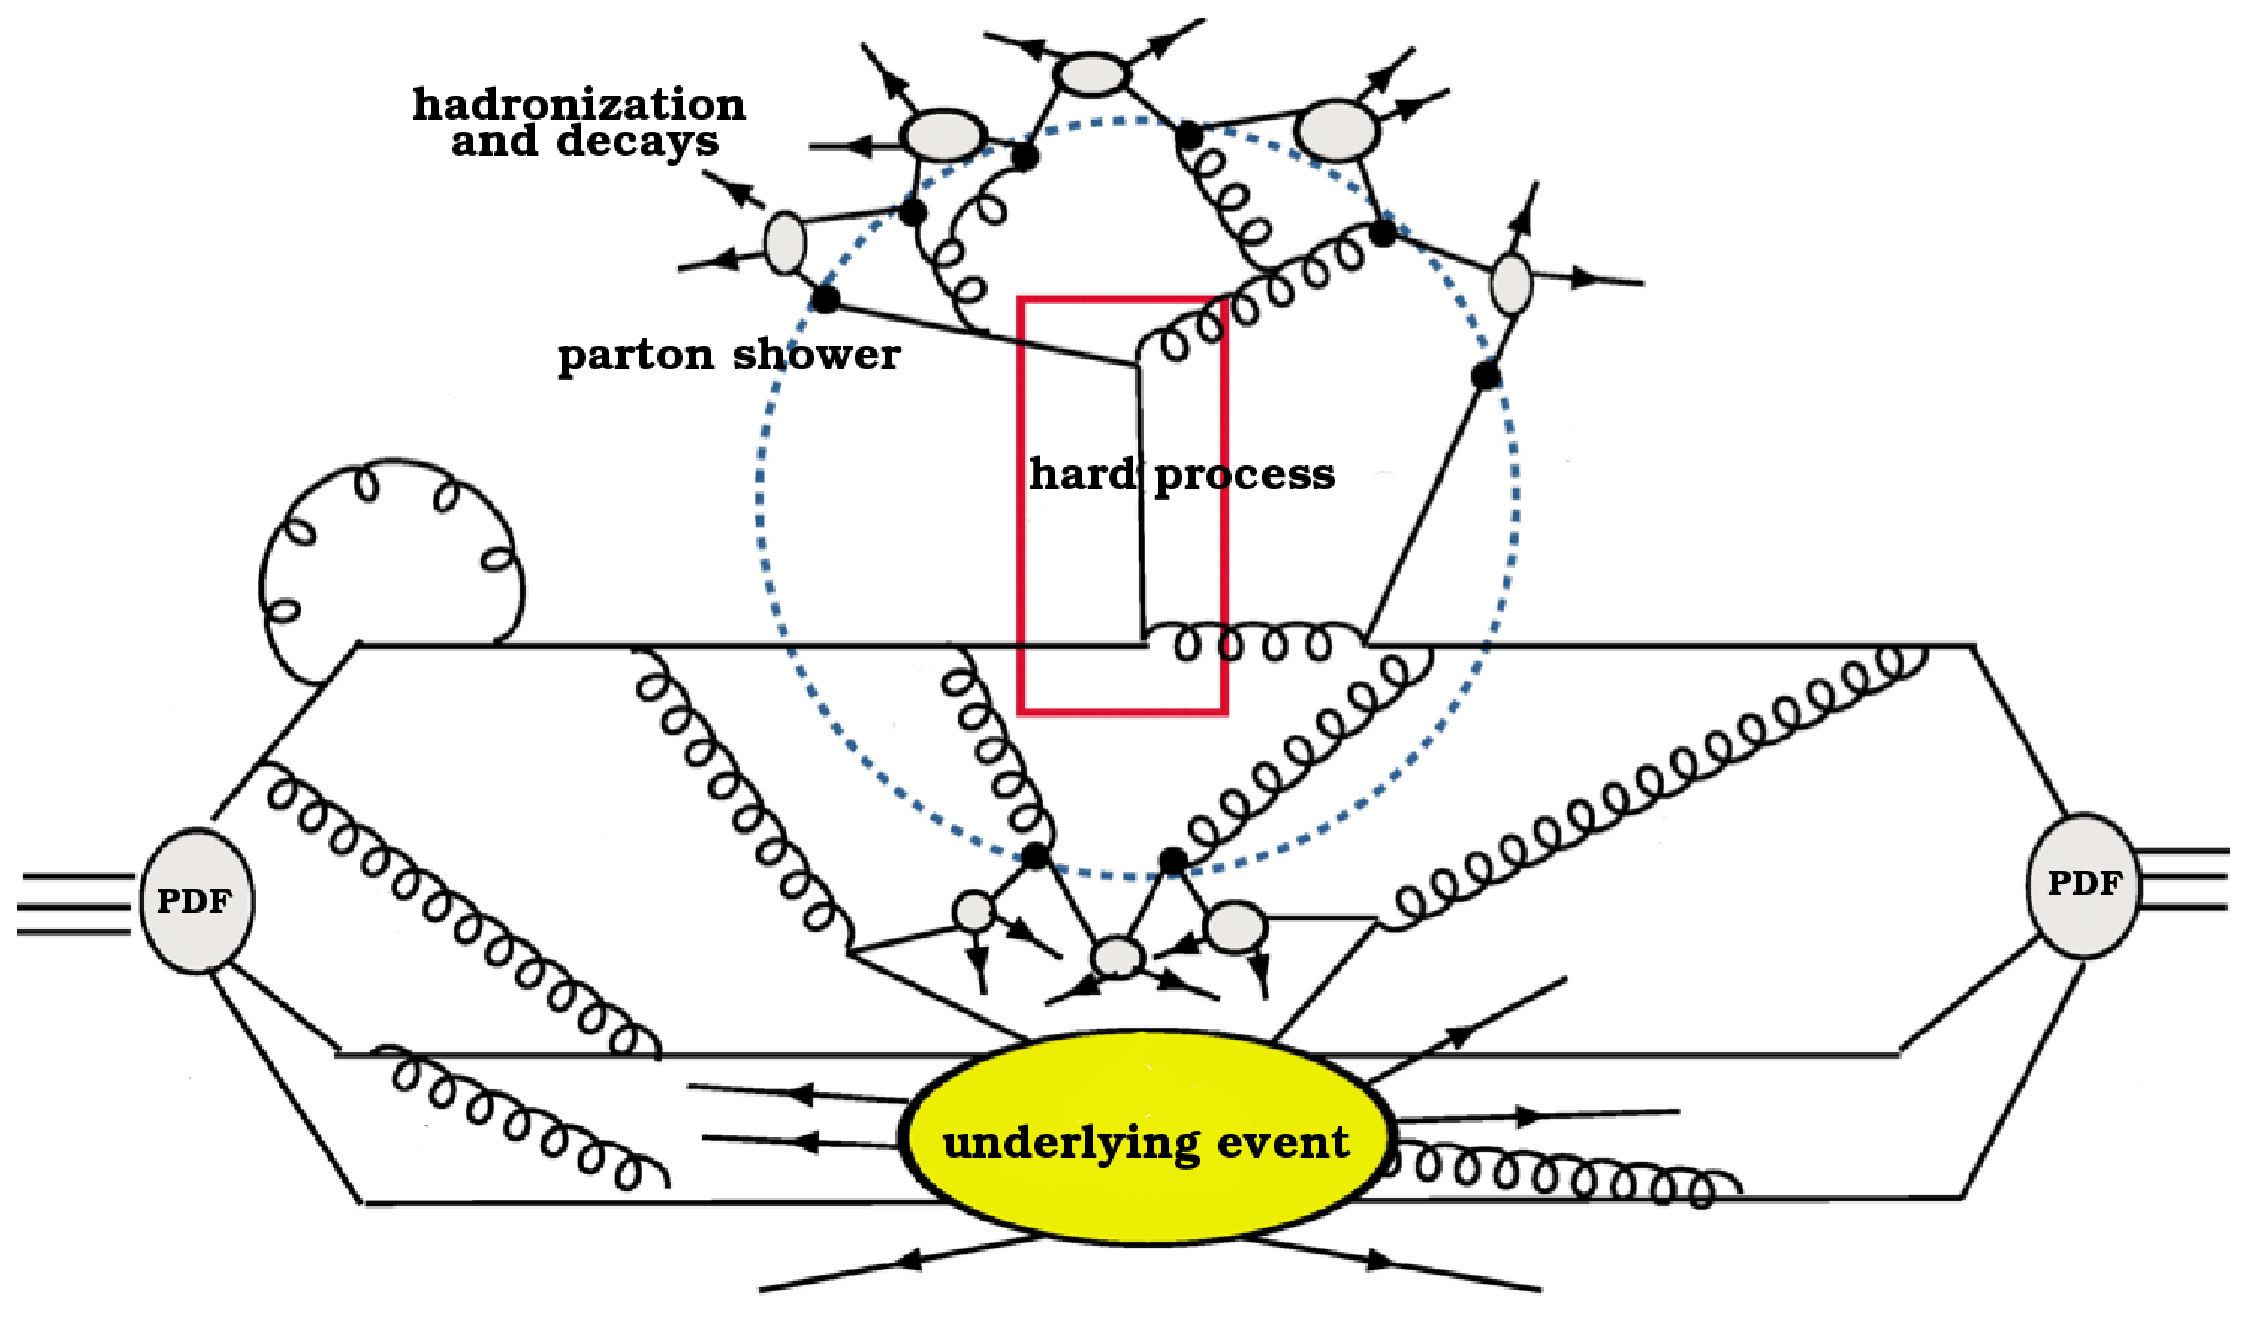
\includegraphics[width=0.8\textwidth]{montecarlo/figures/my_collision}
}
\caption{Drawing describing a hadron-hadron collision from the Monte Carlo
point of view. Partons from the hadron share its energy according to the PDFs. 
The dotted circle separates pQCD events (hard scattering 
and initial and final state radiation) from non-perturbative effects (parton shower, 
hadronization, initial emissions included in the PDFs, and underlying event)\cite{Mangano:933464}.\label{fig:collision}}
%\end{center}
%\end{figure}
%\begin{figure}[htb]\begin{center}
	\subfigure[]{\label{fig:event2}
  	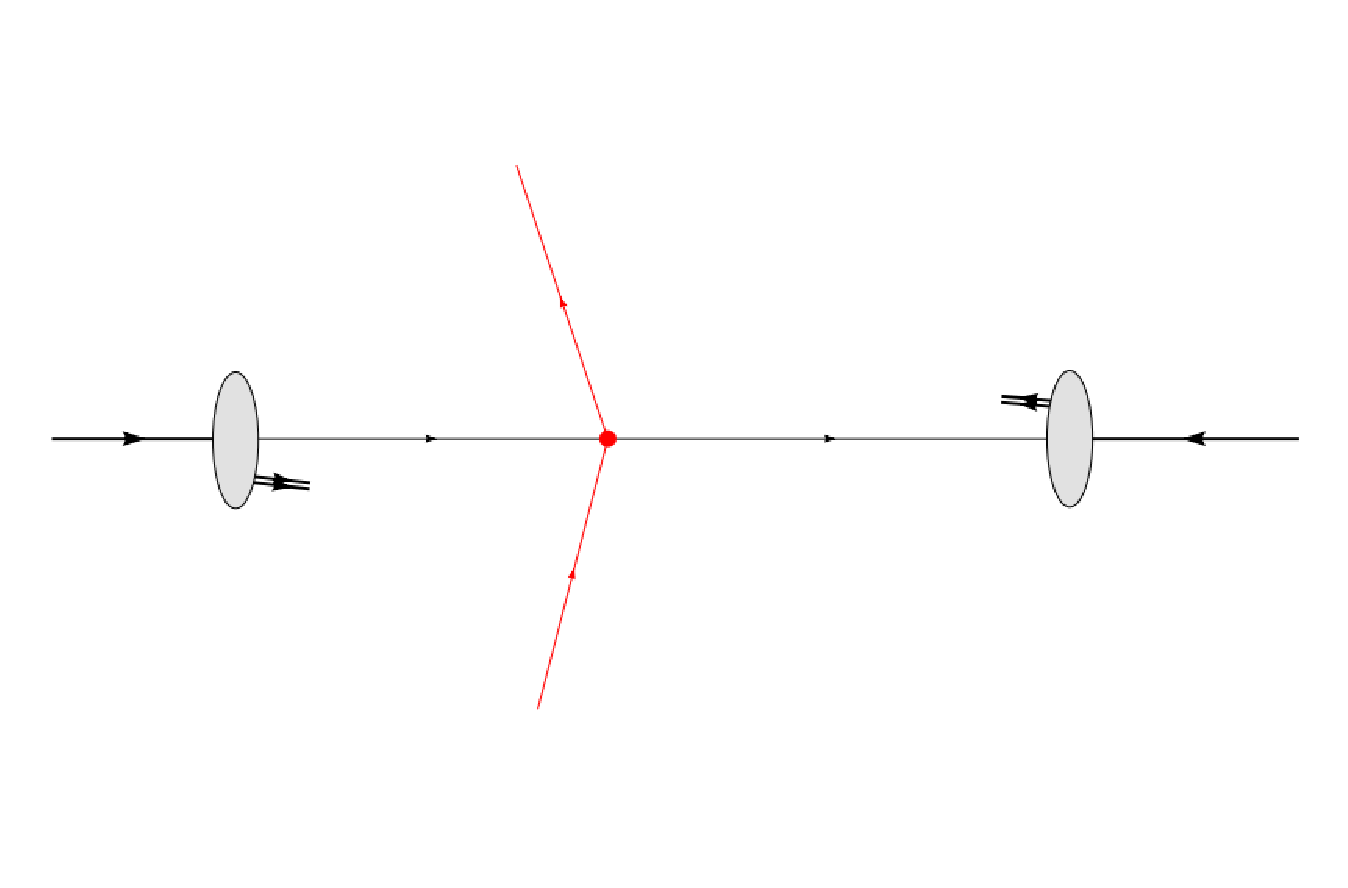
\includegraphics[width=0.45\textwidth,height=0.25\textwidth]{montecarlo/figures/event2}}
	\subfigure[]{\label{fig:event3}
  	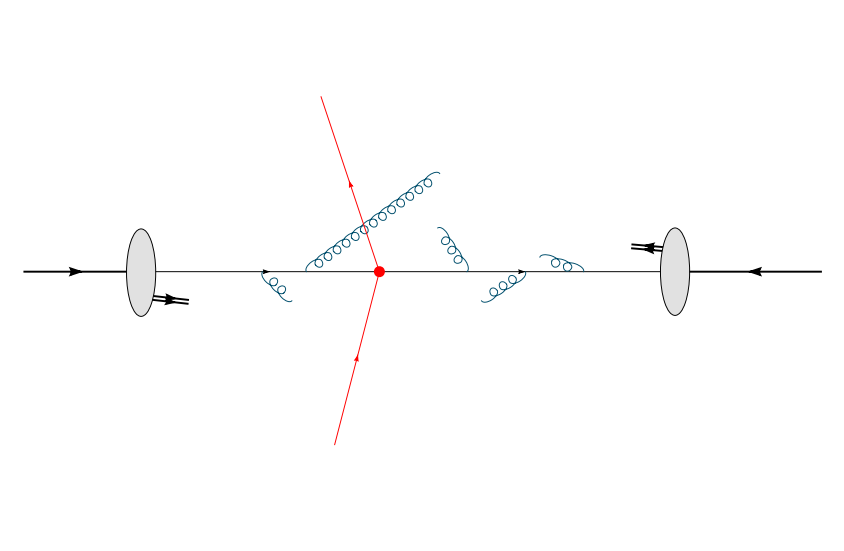
\includegraphics[width=0.45\textwidth,height=0.25\textwidth]{montecarlo/figures/event3}}\\
	\subfigure[]{\label{fig:event4}
  	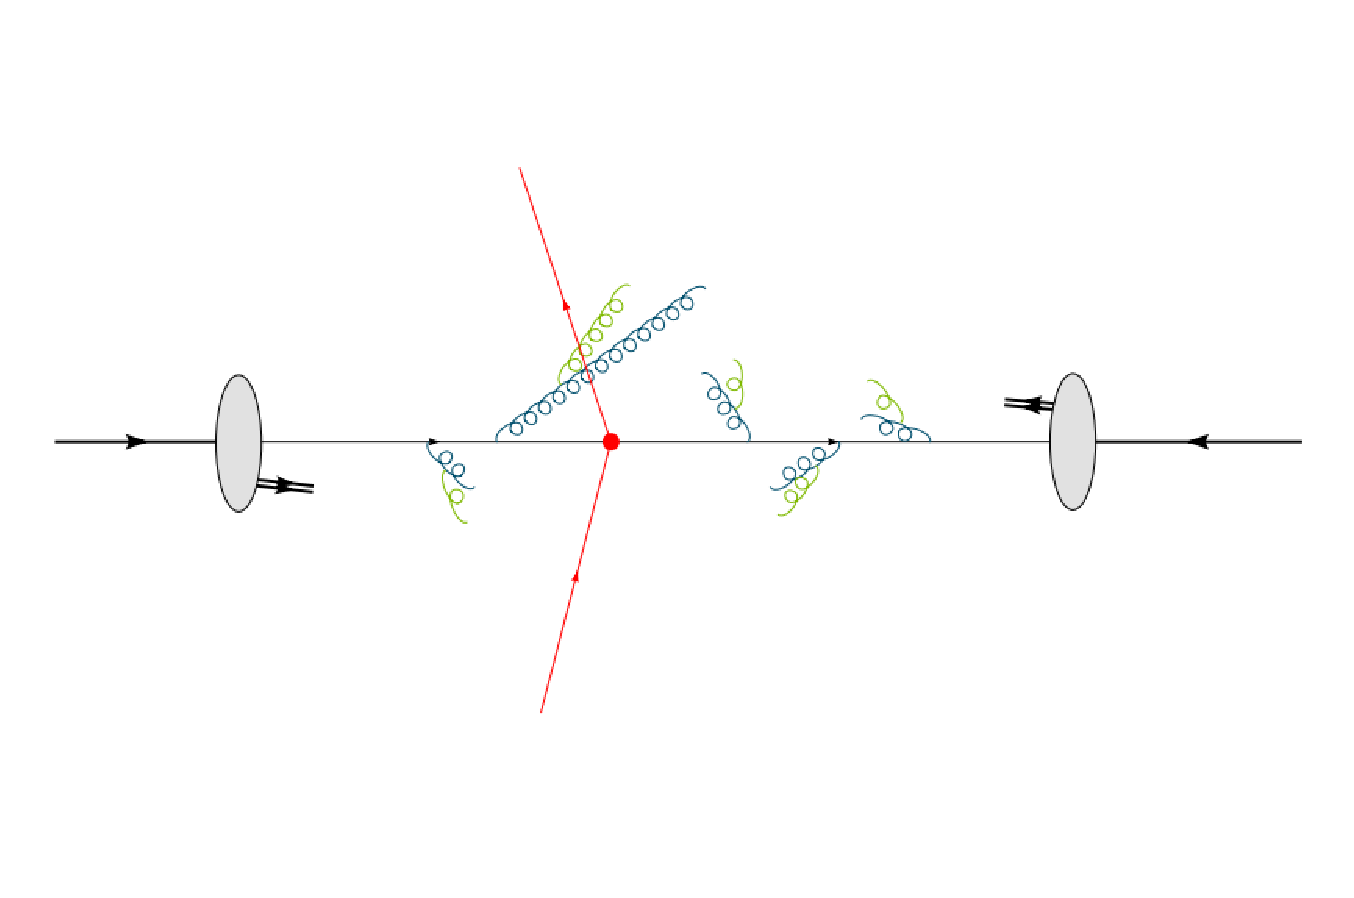
\includegraphics[width=0.45\textwidth,height=0.25\textwidth]{montecarlo/figures/event4}}
	\subfigure[]{\label{fig:event5}
  	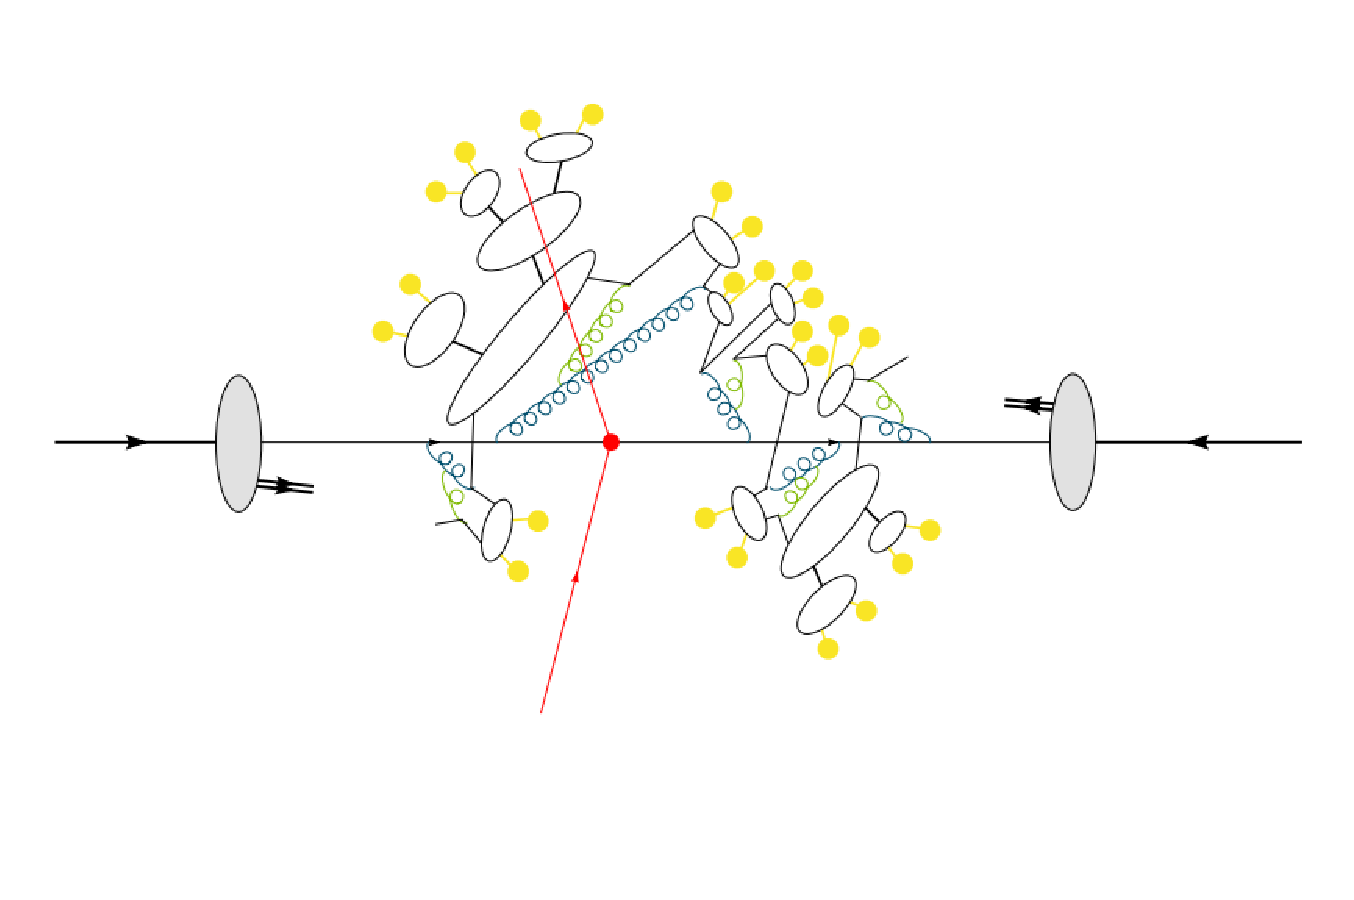
\includegraphics[width=0.45\textwidth,height=0.25\textwidth]{montecarlo/figures/event5}}\\
	\subfigure[]{\label{fig:event6}
  	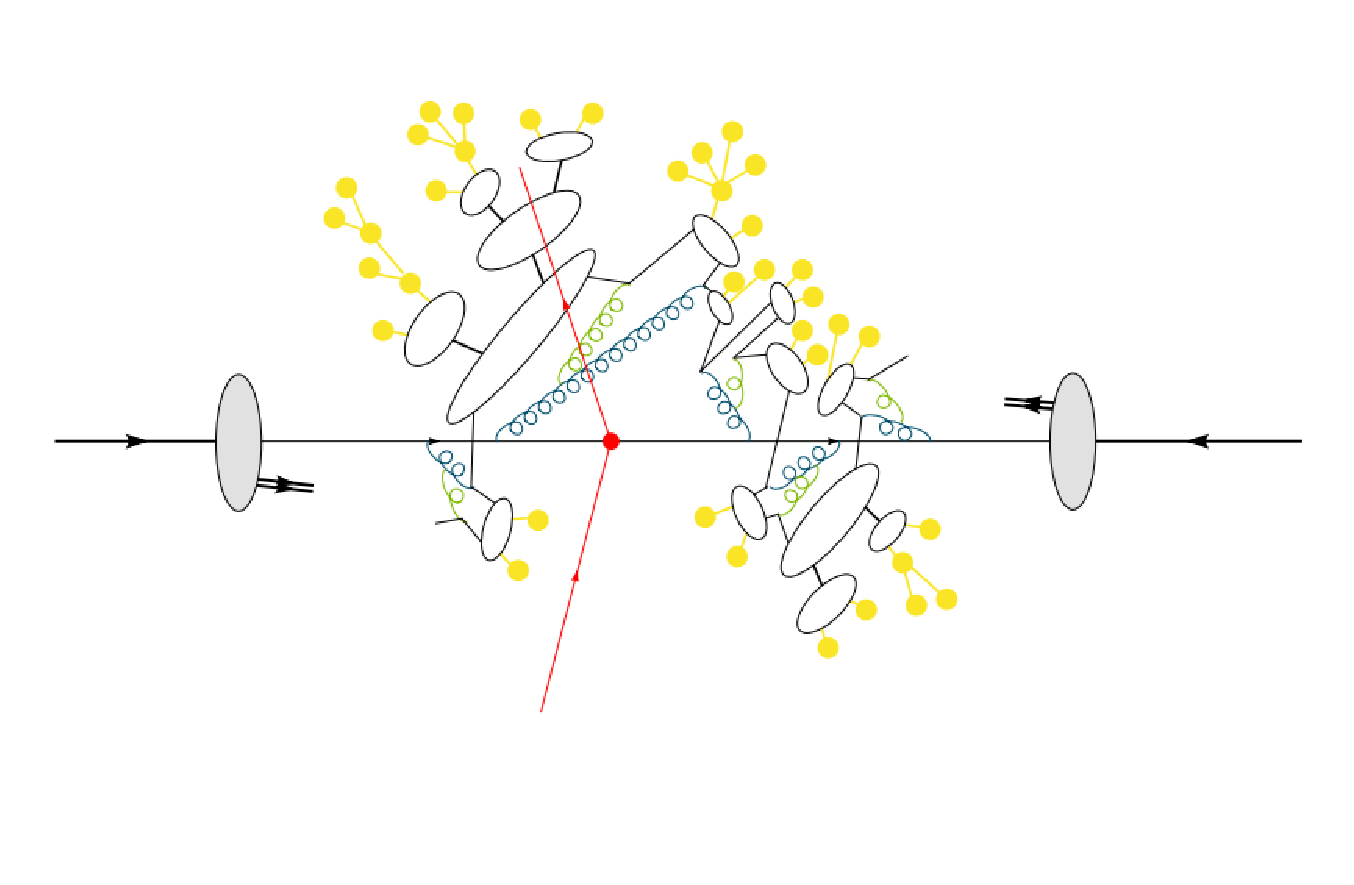
\includegraphics[width=0.45\textwidth,height=0.25\textwidth]{montecarlo/figures/event6}}
	\subfigure[]{\label{fig:event7}
  	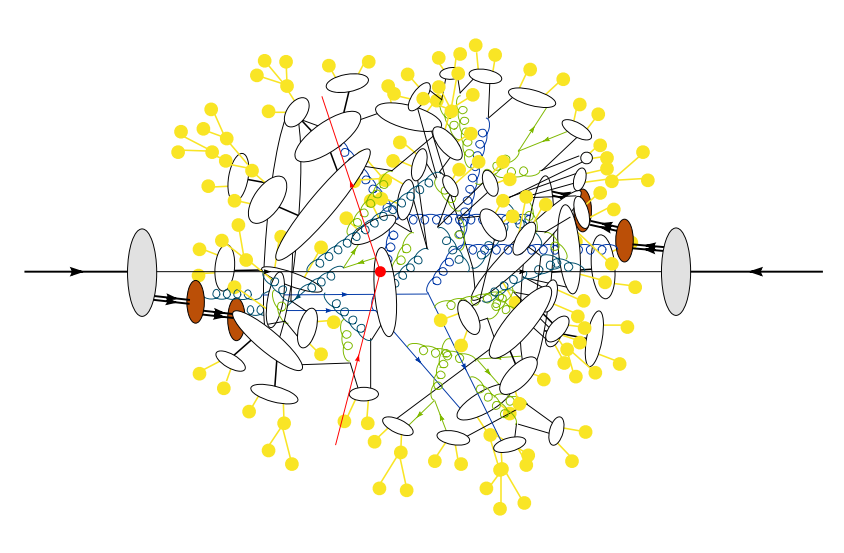
\includegraphics[width=0.45\textwidth,height=0.25\textwidth]{montecarlo/figures/event7}}
	\caption{Set of frames of Monte Carlo event generation evolution: (a) hard scattering of two
        partons; (b) and (c) parton showering; (d) hadronization; (e) final particle decays; (f)
        underlying event simulation. Drawings from~\cite{Gieseke}.\label{fig:eventevolution}}%\footnotemark.}
\end{center}\end{figure}

%\footnotetext{Taken from the slides: \url{http://th-workshop2009.desy.de/e59393/e59379/infoboxContent59381/Gieseke.pdf}.}


\subsection{Hard interaction}\label{sec:matrixelement}

Recalling what discussed in Section~\ref{sec:factorization} about the computation in pQCD
of the hard scattering cross section of a typical LHC $pp\to X$ event, we can rewrite
Equation~\ref{eq:QCDCrossSection} as:
\begin{equation}
\begin{split}
  \sigma_{{\rm pp}\to{\rm X}}
  & = \sum_{a,b}%~\in~{\rm partons}}
  \int{\rm d}x_a{\rm d}x_b
  ~ \int
  ~ f_a(x_a,\mu_{F}) f_b(x_b,\mu_{F})
  {\rm d}\hat{\sigma}_{\rm ab}(x_ap_a, x_bp_b,\mu_R,\mu_{F}) \\
  & = \sum_{a,b}%~\in~{\rm partons}}
  \int{\rm d}x_a{\rm d}x_b
  ~ \int{\rm d}\Phi_{\rm X}
  ~ f_a(x_a,\mu_{F}) f_b(x_b,\mu_{F})
  ~ \times \dfrac{1}{2x_ax_bs}\big|\mathcal{M}_{\rm ab}\big|^2(\Phi_{\rm X},\mu_R,\mu_{F}),  \\
\end{split}
\label{eq:matrixelement1}
\end{equation}
where we introduced the dependence on the final state phase space $\Phi_{\rm X}$, the parton flux
$\frac{1}{2x_ax_bs}$ (with $s$ being the pp \cme\ squared) and the {\it matrix element} $|\mathcal{M}_{\rm ab}|$
for the event of interest.
%which is also written as a sum over Feynman diagrams:
%\begin{equation}\label{eq:matrixelement2}\mathcal{M}_{\rm ab} = \sum_i \mathcal{F}^{(i)}_{\rm ab}.\end{equation}

%presence of collinear and soft divergences in fixed order calculations with a definite final state. Only by summing over different final states these divergences can cancel, thereby allowing the computation of certain (i.e. the collinear and infrared insensitive) inclusive quantities. The only frameworks in which exclusive quantities can be computed must involve the resummation of an infinite class of Feynman graphs. 



\subsection{Parton shower}\label{sec:partonshower}

The parton shower algorithm adds higher-order corrections 
to the hard scatter in an approximative way,
since real radiative corrections to any inclusive quantity (like the hard cross section as computed at
fixed order in pQCD) are divergent. The dominant contributions below a cut-off parameter, associated to 
collinear parton splitting or soft gluon emission, are included iteratively ordered in sequence of, typically, smaller emission angles.
%The Kinoshita-Lee-Nauemberg theorem assures that virtual corrections cancel.

There are three possible processes for QCD emission: 
$q\to gq$, $g\to gg$ and $g\to q\bar{q}$.
The cross section then factorizes into the product of 
the parent parton production cross section times
 a splitting factor. Considering e.g. the $q\to gq$ 
splitting from a tree level process with $n+1$
final state particles we can graphically represent it as
in Figure~\ref{fig:factorization}, with the quark and the
gluon (with four-momenta $k$ and $l$ respectively) 
being emitted at a small angle $\theta$.
Mathematically we have:
\begin{equation}
  \big|\mathcal{M}_{n+1}\big|^2{\rm d}\Phi_{n+1} \to 
  \big|\mathcal{M}_{n}\big|^2{\rm d}\Phi_{n} \dfrac{\alphas}{2\pi}\dfrac{{\rm d}t}{t}P_{q,qg}(z)\dfrac{{\rm d}\phi}{2\pi},
\label{eq:splitting1}
\end{equation}
where $\phi$ is the azimuth defined by $\vec{k}$ and 
$\vec{l}$ around the $\vec{k}+\vec{l}$
direction, $z$ is an arbitrary parameter in general defined as a ratio between the
energy of the particles emitted,
$z = k^0/(k^0 + l^0)$,
and $t$ is the {\it hardness} parameter characterizing the divergence
and the ordering of the splittings. It has the dimensions of a mass
squared, and 
the preference is to take it as $t = E^2\theta^2$. 
The values for $\phi$, $z$ and $t$ are generated randomly during the Monte
Carlo simulation process. 
The function $P_{q,qg}(z)$ is
the Altarelli-Parisi splitting function
which describes the probability for a quark to emit a gluon,
 and is the only term that changes in
Equation~\ref{eq:splitting1} between $q\to gq$, $g\to gg$ and $g\to q\bar{q}$ 
splittings.

\begin{figure}[hbt]\begin{center}
	\subfigure[]{\label{fig:factorization}
  	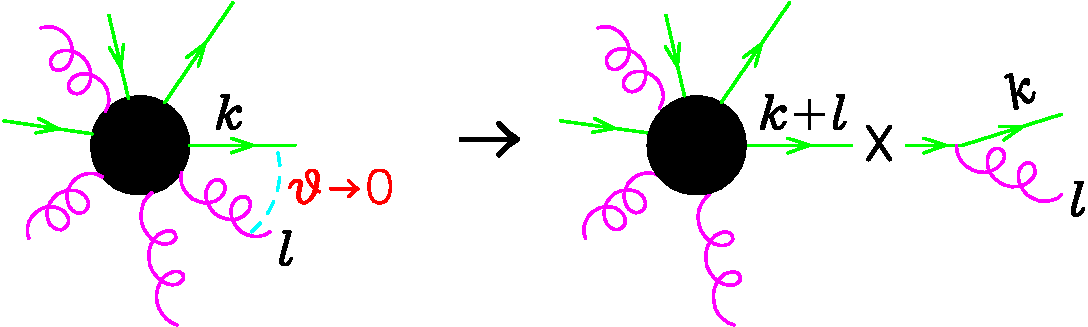
\includegraphics[width=0.45\textwidth]{montecarlo/figures/factorization}}\hskip5ex
	\subfigure[]{\label{fig:splitkin}
  	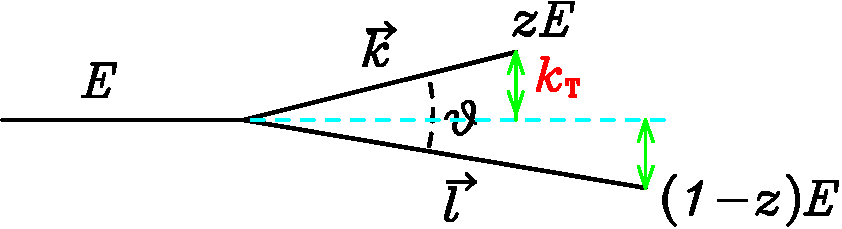
\includegraphics[width=0.4\textwidth]{montecarlo/figures/splitkin}}
	\caption{Left: graphical representation of the $q\to qg$ splitting. The
        black circles represent the $\mathcal{M}_{n+1}$ and $\mathcal{M}_{n}$
        amplitudes of the tree-level processes. Right: kinematic of the splitting~\cite{Ambroglini:2009nz}.}
\end{center}\end{figure}

Factorization holds if the virtuality of the splitting parton $q^2 = (k+l)^2$ 
is negligible with respect to the energies entering the process, and 
can be applied iteratively as shown graphically in Figure~\ref{fig:factorization2}.
At this point, allowing for $n$ splitting processes, the cross section can be written as:
\begin{equation}
  \label{eq:leadinglog} 
  %\sigma_0 \alpha_S^n \int \frac{d t_1}{t_1}  \frac{d  t_2}{t_2} \ldots \frac{d t_n}{t_n} \times \theta (Q^2 > t_1 > t_2 > \ldots >  t_n > \lambda^2) = 
  \sigma_0 \frac{1}{n!} \alpha_S^n \log^n
  \frac{Q^2}{\lambda^2},
\end{equation}
where $Q$ is the upper cut-off scale called {\it annihilation energy} that determines
when the showering starts, and $\lambda$ is the infrared cut-off. The shower ends
when the virtuality $q^2$ reaches the {\it hadronization scale}, which is of the
order of $1~\gev^2$. From the cross section expression of Equation~\ref{eq:leadinglog},
this procedure is called ``leading log approximation''.

\begin{figure}[tb]\begin{center}
	\subfigure{
  	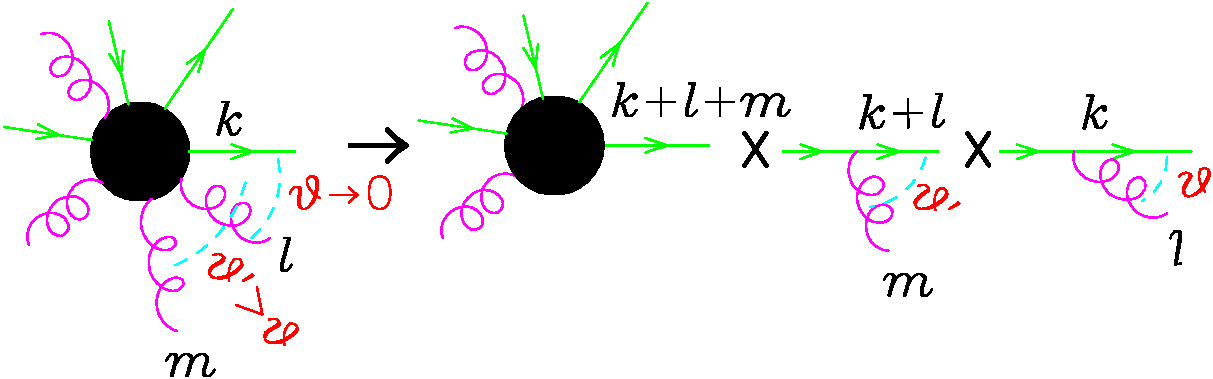
\includegraphics[width=0.6\textwidth]{montecarlo/figures/factorization2}}
	\caption{Recursive application of factorization, with the angles ordered
        as  $\theta' \gg \theta \rightarrow 0$~\cite{Ambroglini:2009nz}.\label{fig:factorization2}}
\end{center}\end{figure}

Once the shower is developed, the vertices and lines of the final configuration are
assigned weights, which are for each vertex:
  \begin{equation}
    \label{eq:splitvert} \theta (t - t_0) \hspace{0.75em} \frac{\alpha_S
    (t)}{2 \pi} \hspace{0.25em} \frac{dt}{t} \hspace{0.25em} P_{i, j l} (z)
    \hspace{0.25em} dz \hspace{0.25em} \frac{d \phi}{2 \pi},
  \end{equation}
and for each line are the so-called {\it Sudakov form factors}:
  \begin{equation}
    \label{eq:sudadef} \Delta_i (t', t'') = \exp \left[ - \sum_{(j l)}
    \int_{t''}^{t'} \frac{dt}{t} \int_0^1 d z \hspace{0.75em} \frac{\alpha_S
    (t)}{2 \pi} \hspace{0.25em} \hspace{0.25em} P_{i, j l} (z) \right]
  \end{equation}
where $t'$ is the value of $t$ at the upstream vertex, and $t''$ 
at the downstream vertex. If we reached the end of the graph,
$t''$ is substituted by a cut-off $t_0$.
The Sudakov form factors specify the range of the $z$ parameter for 
which the splitting is resolvable and represent the probability
of {\it not} splitting. Figure~\ref{fig:showergraph} shows
the typical graph shape of a shower evolved with splittings
strongly ordered in angle.

\begin{figure}[hbt]\begin{center}
	\subfigure{
  	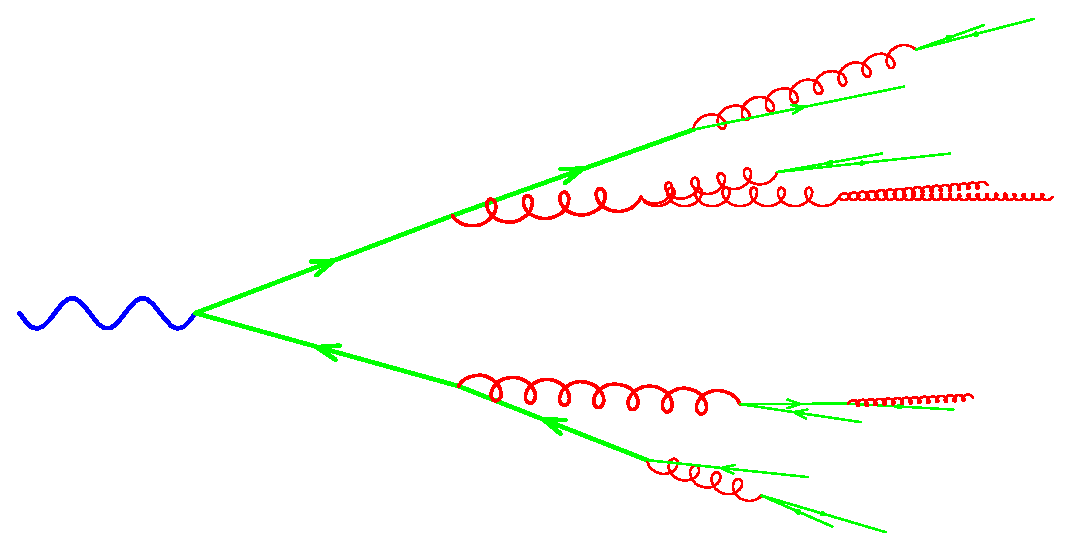
\includegraphics[width=0.6\textwidth]{montecarlo/figures/MCWSShower}}
	\caption{An example of a typical shower final graph~\cite{Ambroglini:2009nz}.\label{fig:showergraph}}
\end{center}\end{figure}

\subsubsection{Initial- and final-state radiation}\label{sec:isrfsr}

Up until now we have discussed the development of the parton shower arising
from the emission from hadrons produced in the hard scattering, i.e. 
starting in general at a high energy scale $Q^2$ and progressively
reaching the hadronization scale. This process goes under the name of
{\it final state radiation} (FSR), as it is generated from outgoing
partons of the hard interaction.

Parton showering can of course also happen before the hard interaction, and
is called {\it initial state radiation} (ISR) as the incoming partons
of the hard scattering originate the emission. In this case
there is an important difference in the shower evolution, that is
that the final energy of the showering is the hard interaction energy
scale. To respect this fact, Monte Carlo simulation of ISR adopts a 
``backward evolution'', first setting the correct parton momentum distributions
for the hard scatter, and then developing the shower backward, with the 
intermediate partons aquiring energy at each emission. The Sudakov form 
factors are then slightly different from Equation~\ref{eq:sudadef}, being
rescaled by a factor that takes into account the PDFs of the parton at the
two vertices.


\subsubsection{Matrix element and parton shower matching}\label{sec:matching}

We have introduced two powerful ways to describe a QCD event, one relying
on our capability to compute the Matrix Elements (ME) in pQCD at the LO and NLO,
the other exploiting a procedure to develop Parton Showers (PS) including
soft and collinear emissions. ME calculations can also describe soft and collinear emissions,
but the ME weight is in this case divergent, while in the PS scheme divergences
are eliminated through the Sudakov form factors. We need therefore to set 
the rules to conveniently split the phase space of the event into two regions,
one characterized by hard and large-angle emission to be described by ME, the
other of soft and collinear emission to be described by the PS. This is achieved
in the so-called ``ME and PS matching'', where some resolution parameters are
introduced with the role of serving as soft and collinear cut-offs for the ME. 

The basic idea is to compute the weight of an event using ME and then
develop PS giving as inputs the ME weight as well as the event kinematics and 
color flow. A complication arises in this simple approach as the same final
state can be obtained in multiple ways if ME and PS generated partons are swapped,
as graphically shown in Figure~\ref{fig:matchfig1}, where the same event 
has three possible configurations. This issue is referred to as ``double
counting'', and the aim of the matching scheme is to avoid it.

\begin{figure}[htb]\begin{center}
	\subfigure{
  	\includegraphics[width=0.7\textwidth]{montecarlo/figures/matchfig1}}
	\caption{Example of double counting in hadron production. Dashed lines
        are PS emissions, solid lines are ME emissions. On the left, we have one
        hard large angle emission from ME and soft collinear emissions from PS.
        In the middle and on the right, one soft collinear emission from ME 
        and both hard and soft PS emissions~\cite{Ambroglini:2009nz}.
        \label{fig:matchfig1}}
\end{center}\end{figure}

The main requirements on the matching scheme, besides avoiding double counting,
are also to perform a smooth transition from the ME to the PS regions and to make
sure the appropriate Sudakov form factors reabsorb the divergencies eventually
introduced by the ME by reweighting the ME weight.

There are two main matching schemes: the Catani-Krauss-Kuhn-Webber 
(CKKW~\cite{Catani:2001cc}) and the Michelangelo L. Mangano 
(MLM~\cite{Mangano:2006rw}) methods.
They separate the phase space into the ME and PS regions by
introducing resolution parameters that distinguish between
{\it resolved} and {\it non-resolved} jets, to be described by
means of the ME and PS respectively.

In the CKKW scheme, the parton-parton separation is measured by defining
the distances between two final state partons and the distance between the 
parton and the beam using the $k_\perp$ jet algorithm~\cite{Catani1991432}. 
For a parton to be resolved, and described through ME,
both variables have to be greater than a resolution parameter $Y_{\rm sep}$. 
A branching tree is developed clustering together the two closest partons
and  ME elements are reweighted first to the strong coupling \alphas\ value 
at the ME scale and then using a combination of Sudakov form factors.
Then, PS is evolved and emissions at scales greater than 
$Y_{\rm sep}$ are vetoed, thus avoiding overlap between configurations. 

In the MLM scheme, partons are first clustered into samples with different 
multiplicity and then, like in the CKKW method, the $k_\perp$ jet algorithm
is used to develop a branching tree and ME are reweighted to the proper strong 
coupling \alphas\ value. At this point PS is performed and a jet finding algorithm
matches partons into clusters. Jets with 
$p_T>p_{T_{\rm min}}$, separation $R>R_{\rm min}$ and 
pseudorapidity $\eta<\eta_{\rm max}$ are considered for matching 
partons. Events are kept only if there is a one-to-one correspondence 
of partons to jets, else is rejected and thus double counting is avoided.
As final step, the ME is reweighted with a Sudakov form factor.

The performance of the two matching methods has been extensively tested
with data, and in particular it is important that the independence of
the final result from the resolution parameters is verified.


\subsection{Hadronization}\label{sec:hadronization}

When partons reach the hadronization scale energy $Q\sim 1\gev$ after showering,
they recombine in colorless bound states according to the confinement
principle, holding at low momentum. The so-called {\it parton-hadron duality}
assumes that no high momentum transfer is needed in the recombination,
as it happens  close in phase space. This is a property of QCD
experimentally observed, but there are no theoretical arguments
explaining the hadronization. The solution is then to rely on
phenomenological models.

The principle at the basis of hadronization models used in Monte Carlo is the 
{\it large $N_c$ limit}, or {\it planar limit}, where $N_c$ is the number
of colors and we consider the QCD value $N_c = 3$ as just the dominant
contribution. Simple rules are then defined: color and anticolor indices
go from 1 to $N_c$; quark and antiquark lines are oriented and assigned
a color and anticolor index respectively; gluon lines are oriented and assigned
a pair of color-anticolor indices to achieve color neutrality. 
The color structure of the three splitting
processes according to these rules are shown in Figure~\ref{fig:planarrules}.
While the assignment of color connections in the case of $q\to qg$ and
$g\to q\bar{q}$ splittings is univocal, for $g\to gg$ there are two possible
configurations (where by inverting the two final state gluons transform one
into the other) and when the color connections are reconstructed they are chosen
with a 50\% probability each. The final picture looks e.g. like the graph
in Figure~\ref{fig:colourflow}, where the important information is not the
specific color assigned to the final state parton, but rather the {\it color flow}.


\begin{figure}[hbt]\begin{center}
	\subfigure[]{\label{fig:planarrules}
  	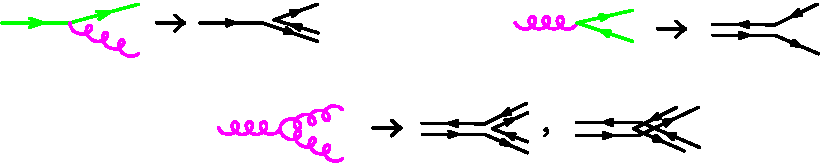
\includegraphics[width=0.45\textwidth, height=0.18\textwidth]{montecarlo/figures/planarrules}}\hskip5ex
	\subfigure[]{\label{fig:colourflow}
  	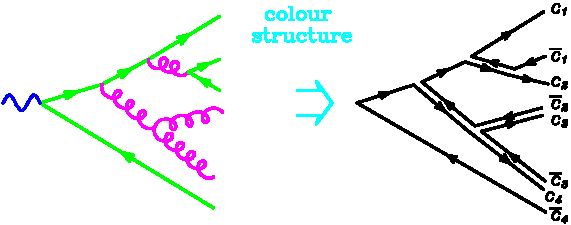
\includegraphics[width=0.45\textwidth]{montecarlo/figures/colour2}}
	\caption{Left: rules to assign color connections in the splittings
        $q\to qg$ (top left), $g\to q\bar{q}$ (top right) and $g\to gg$ 
        (bottom). Right: example of a color connected shower~\cite{Ambroglini:2009nz}.}
\end{center}\end{figure}

At this point, two possible phenomenological fragmentation models are typically used
to bound partons into hadrons starting from the color-connected final state. 
%They both have been tuned using collider measurements over the last decades
%to properly describe the final state hadron multiplicity and need in general
%a large number of parameters.

The first hadronization scheme is called {\it Lund string model} and ties a quark
with an antiquark plus a number of intermediate gluons, like
stretching a string (or a ``color flux tube'') from the quark
to its color-connected antiquark taking in the gluons that
lie in between them. This can be see as an illustration in 
Figure~\ref{fig:had_colorflow} and Figure~\ref{fig:had_string}:
the first string collects the quark with color $c_1$, the antiquark
with color $\bar{c}_4$ and all the final state gluons along the path.
 uses string dynamics to describe the color flux between quarks. 
In other words, the string between the quark and antiquark produces a linear
confinement potential.

The other hadronization scheme is the {\it cluster model}, where
final state gluons are forced to split into a quark-antiquark pair
and then color connected quark-antiquark pairs are bounded together.
Figure~\ref{fig:had_cluster} presents a graphical illustration of the
concept. Because of {\it preconfinement} (the fact that color connected pairs
with large invariant masses are Sudakov suppressed in angular ordered showers)
the cluster can be associated with a hadronic two-body system. 

During the last decades, different measurements at colliders have
been used to tune these models to properly describe 
the hadron multiplicity in the final state,
and need in general a large number of parameters.



\begin{figure}[hbt]\begin{center}
	\subfigure[]{\label{fig:had_colorflow}
\def\svgwidth{0.3\textwidth}
\input{montecarlo/figures/had_colorflow.eps_tex}}
	\subfigure[]{\label{fig:had_string}
  	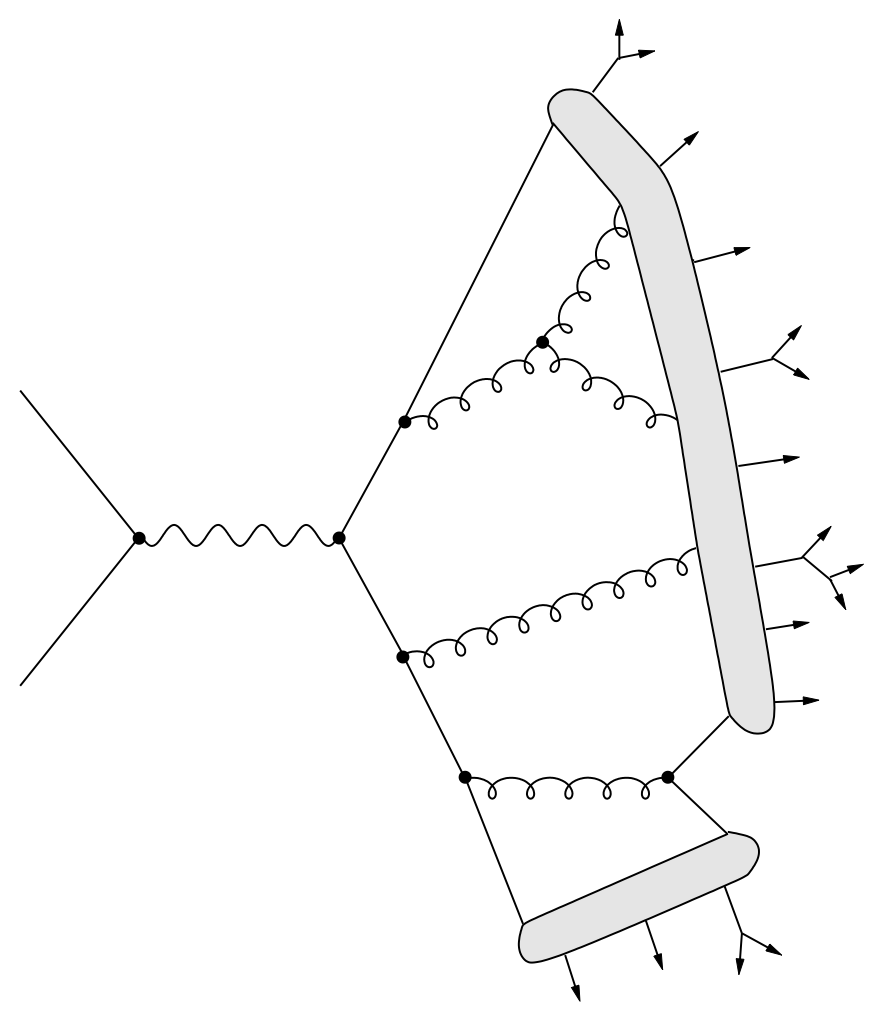
\includegraphics[width=0.3\textwidth]{montecarlo/figures/had_string}}
	\subfigure[]{\label{fig:had_cluster}
  	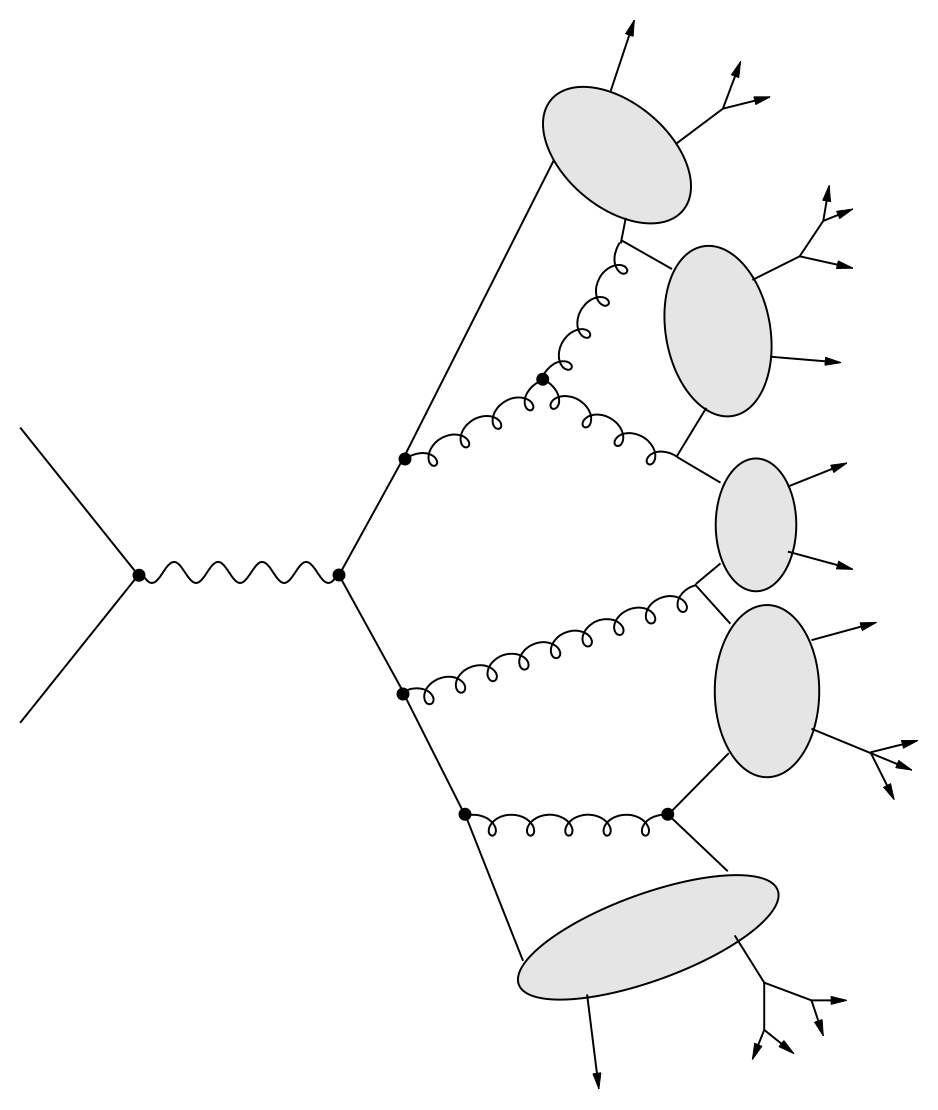
\includegraphics[width=0.3\textwidth]{montecarlo/figures/had_cluster}}
	\caption{Drawing of a color connected parton shower graph (a) completed with hadronization from the Lund string model (b) and the cluster model (c)~\cite{Mangano:933464}.}
\end{center}\end{figure}



\subsection{Underlying event}\label{sec:underlyingevent}

With ``underlying event'' (UE) we refer to the secondary parton interactions 
at low momentum transfer that accompany the main hard process. 
The underlying event is flavor- and color-connected to the hard scattering
and in real data is in general not separable from the event of interest.
It is typically observed as jets of particles close to the direction
of the beam and cannot be modeled with perturbative QCD.
% but is instead studied from experimental data on {\it minimum bias} events at low momentum.

Besides a backward shower modeling starting from the beam remnants, an
important contribution to the underlying event are multiple parton interactions,
i.e. secondary relatively hard collisions between the incoming hadron remnants.
Phenomenological models are used to simulate the underlying event
and are tuned to {\it minimum bias}\footnote{A ``bias'' in event selection
is, in general, any kind of assumption made on the final state and therefore
any kind of cut applied in selecting only these events. In minimum bias events
only very loose requirements are imposed on the collision data.} % These events are useful to study the UE since} 
data from hadron colliders. Indeed processes involving IR divergences 
have free parameters that can (must) be phenomenologically constrained.
Hadronization models typically have 10 to 30 free parameters, 
Multi-Parton Interaction (MPI) models usually add at least 5 more
free parameters. An example of these studies is given in 
Figure~\ref{fig:minbiastune}, where ATLAS tunes for \texttt{PYTHIA6}
are compared to minimum bias event data. More details can be found
in Reference~\cite{Buckley:2011vq}.

\begin{figure}[htb]\begin{center}
	\subfigure[]{
  	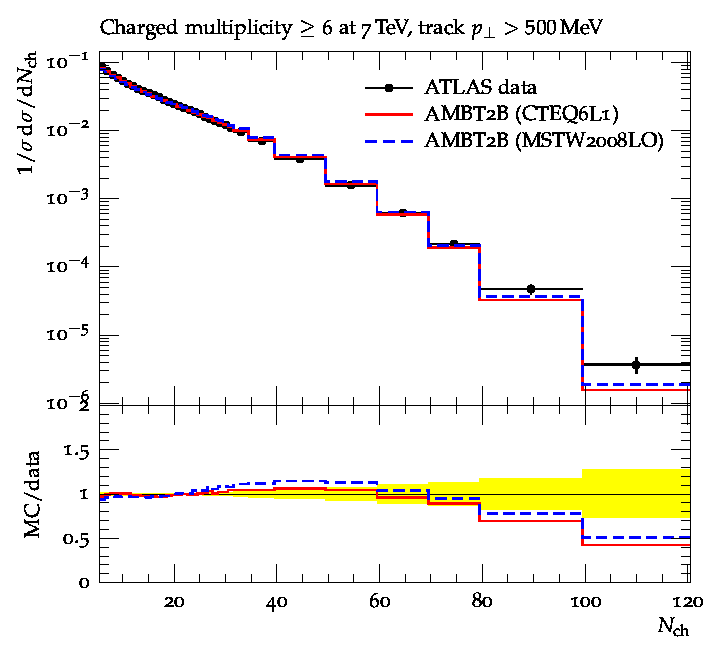
\includegraphics[width=0.45\textwidth]{montecarlo/figures/py6/ATLAS_MINBIAS_MB20_d06-x01-y01.eps}}
	\subfigure[]{
  	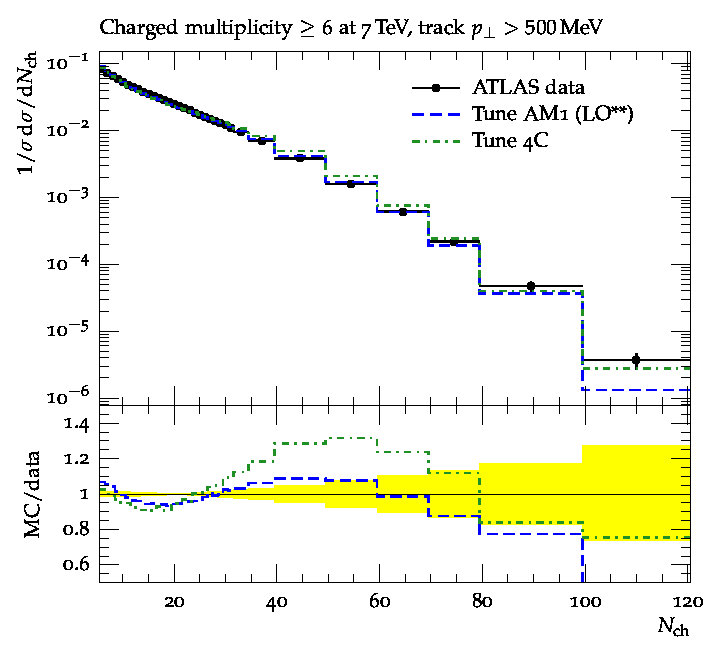
\includegraphics[width=0.45\textwidth]{montecarlo/figures/py8/d06-x01-y01.eps}}
	\caption{Charged particle multiplicity distributions comparing ATLAS
        data from minimum bias events at a \cme\ of 7~\tev\ 
        with  \texttt{PYTHIA6} (a) and  \texttt{PYTHIA8} (b) tunes~\cite{Buckley:2011vq}.\label{fig:minbiastune}}
\end{center}\end{figure}


 
%, and additional semi-hard interactions are generated with different primary vertices to account for the effect of pile-up.


\subsection{Pile-up}\label{sec:MCpileup}

In-time pile-up events arise from the multiple parton inelastic scatterings 
of protons in the same bunch of the hadron generating the hard process
of interest. They mainly consist in soft QCD interactions and are
modelled in a similar way as the UE~\cite{Buckley:2011vq,Cacciari:2007fd}. 
Pile-up is also tuned to minimum bias events.


%, and additional semi-hard interactions are generated with different primary vertices to account for the effect of pile-up.



\section{Generators}\label{sec:generators}

Monte Carlo generators can either be {\it multi-purpose} generators,
i.e. capable of performing the full simulation chain described in this chapter,
or {\it specialized} generators, i.e. devoted to a single aspect of the
simulation. As should be clear after the discussion about the modeling
of hadronic collisions, there are some choices to be made that might result
in some generators 
being better suited 
to describe particular processes. Therefore
the Monte Carlo generators should be chosen according to their performance
in modeling the event of interest.

We briefly present in the following sections the main characteristics of the generators
that are used in the analyses that are the object of this dissertation.


\subsubsection*{PYTHIA}

\texttt{PYTHIA}~\cite{PYTHIA,Sjostrand:2007gs} is a multi-purpose Monte Carlo generator
using ME computed at LO for $2 \to n$ ($n\leq 3$) processes and PS with emissions
ordered in $p_T$ instead of angle. The Lund string model is used for hadronization
and UE simulation is included.
% as scattering between proton remnants in  $2 \to 2$ ME computed at LO.
Minimum bias events with $p_T>\hat{\pt}_{min}$ are used to model interactions
between proton remnants.


\subsubsection*{HERWIG}

\texttt{HERWIG}~\cite{HERWIG} is a multi-purpose Monte Carlo generator
using ME computed at LO for $2 \to 2$ processes and PS with emissions ordered in angle. 
The cluster model is used for hadronization and for the UE description, \texttt{HERWIG}
is typically interfaced with the external package \texttt{JIMMY}~\cite{jimmy} which
simulates UE as MPIs in  $2 \to 2$ processes with the ME computed at LO.


\subsubsection*{ALPGEN}

\texttt{ALPGEN}~\cite{ALPGEN} is a Monte Carlo generator specialized for
ME computation of $2 \to n$ ($n\leq 9$) events at LO, with cross sections 
computed using the ALPHA algorithm \cite{ALPGEN_0}. It is interfaced either
with \texttt{PYTHIA} or \texttt{HERWIG} for PS development 
and hadronization, and ME/PS matching
is done in the MLM scheme. %, where the resolution parameter $p_{T_{\rm min}}$ is called {\it jet matching scale}.
UE is simulated through \texttt{HERWIG}
and hence \texttt{JIMMY}.

The various parton multiplicity samples are then normalized to their LO cross section
and combined into an inclusive sample, which is finally typically normalized 
to an inclusive cross section calculated at higher order in pQCD. 
%For the inclusive production of $Z$ and $W$ bosons in pp collisions, the 
%MCFM~\cite{MCFM} and FEWZ~\cite{Gavin:2010az} programs are used to predict 
%cross sections at NLO and NNLO respectively.


\subsubsection*{MC@NLO}

\texttt{MC@NLO}~\cite{mcatnlo} is a Monte Carlo generator simulating ME at
NLO, where the use of 1-loop corrections introduce the possibility of having
negative weighted events. Theoretical uncertainties on the inclusive cross
section is reduced thanks to the use of full NLO corrections, but higher-multiplicity
parton emission beyond the first one is simulated through PS in \texttt{HERWIG} which has
a poorer description of hard emissions. 
Hadronization and UE are also simulated through \texttt{HERWIG}
(and hence \texttt{JIMMY}).

\subsubsection*{SHERPA}

\texttt{SHERPA}~\cite{sherpa} is a multi-purpose Monte Carlo generator
interfaced with \texttt{PYTHIA} for the parton shower. ME/PS matching
is performed with the CKKW scheme.
A modular design for \texttt{SHERPA} allows for  simple implementation
of other techniques, e.g. NLO corrections can be introduced in the
CKKW matching scheme using a NLO Monte Carlo generator with the
\texttt{MENLOPS} procedure~\cite{MENLOPS}.
Hadronization is done within \texttt{PYTHIA} and a multiple parton 
scattering model for UE simulation.


\subsubsection*{POWHEG}

\texttt{POWHEG}~\cite{powheg} is a Monte Carlo generator computing
ME at NLO and typically interfaced either with \texttt{PYTHIA} or 
\texttt{HERWIG} for the modeling of PS, hadronization and UE.
The choice made at the level of interfacing the ME with PS
can lead to large differences in the description of events with
 high jet multiplicity in the final state between \texttt{POWHEG} 
and \texttt{MC@NLO}.

\subsubsection*{MADGRAPH}

\texttt{MADGRAPH}~\cite{madgraph} is a Monte Carlo generator 
specialized for ME computation of $2 \to n$ ($n\leq 6$) events at LO
interfaced with \texttt{PYTHIA} for the modeling of PS within the
MLM matching scheme, and the same for hadronization and UE.


\subsubsection*{ACERMC}

\texttt{ACERMC}~\cite{acermc} is a Monte Carlo generator computing
ME at LO and typically interfaced either with \texttt{PYTHIA} or 
\texttt{HERWIG} for the modeling of PS, hadronization and UE.



\section{ATLAS detector and trigger simulation}\label{sec:MCdetector}

Events generated with Monte Carlo simulation can be directly
used at {\it parton level}, i.e. without any further operation on the
generated partons, or be reconstructed either at {\it particle level}, where
the stable particles\footnote{Stable particles are
defined as to have proper lifetimes longer than 10~ps, excluding
muons and neutrinos.} are used for reconstruction (see Chapter~\ref{chap:objects})
without considering any possible interaction in the detector material, 
or go through detector simulation~\cite{atlas_sim} followed by 
trigger simulation (which in general uses a trigger selection
representative of a given data-taking period~\cite{Galster:1622237}) and finally event
reconstruction, to obtain the so-called {\it reconstructed level} of
physics objects. The scheme presented in Figure~\ref{fig:outline}
shows the ATLAS simulation data flow 

\begin{figure}[htb]\begin{center}
	\subfigure{
  	\includegraphics[width=0.9\textwidth]{montecarlo/figures/outline_v3}}
	\caption{The flow of the ATLAS simulation software, from event generators (top left) through reconstruction (top right).
        The red path leads to {\it particle level} physics objects, the blue path to
        {\it reconstructed level} physics objects, while the green path shows the real data
        flow to physics objects.
        %Algorithms are placed in square-cornered boxes and persistent data objects are placed in rounded boxes. 
        %The optional pile-up portion of the chain, used only when events are overlaid, is dashed. 
        %Generators are used to produce data in HepMC format.  
        %Monte Carlo truth is saved in addition to energy depositions in the detector (hits). 
        SDO stands for Simulated Data Object, ROD for Read Out Driver~\cite{atlas_sim}.\label{fig:outline}}
\end{center}\end{figure}

The detector material, geometry and response %simulation~\cite{atlas_sim} 
are modeled using the {\tt GEANT4}~\cite{geant} package.
This code evolves the particles simulating a real environment
where they can cross volumes of material and leave energy
deposits or hits. Figure~\ref{fig:atlasdisplay} shows an
example of a Higgs boson decay event simulated in the detector
geometry.
The interaction of particles with ATLAS subsystems is converted
into detector signals of the same sort of the real read-out and
at this point the same kind of reconstruction algorithms shape
the detector output into physical objects. During test-beam periods
the \texttt{GEANT4} parameters have been tuned to best simulate
the ATLAS configuration and the performance of detector simulation
has been extensively checked also with data calibrations.

\begin{figure}[htb]\begin{center}
	\subfigure{
  	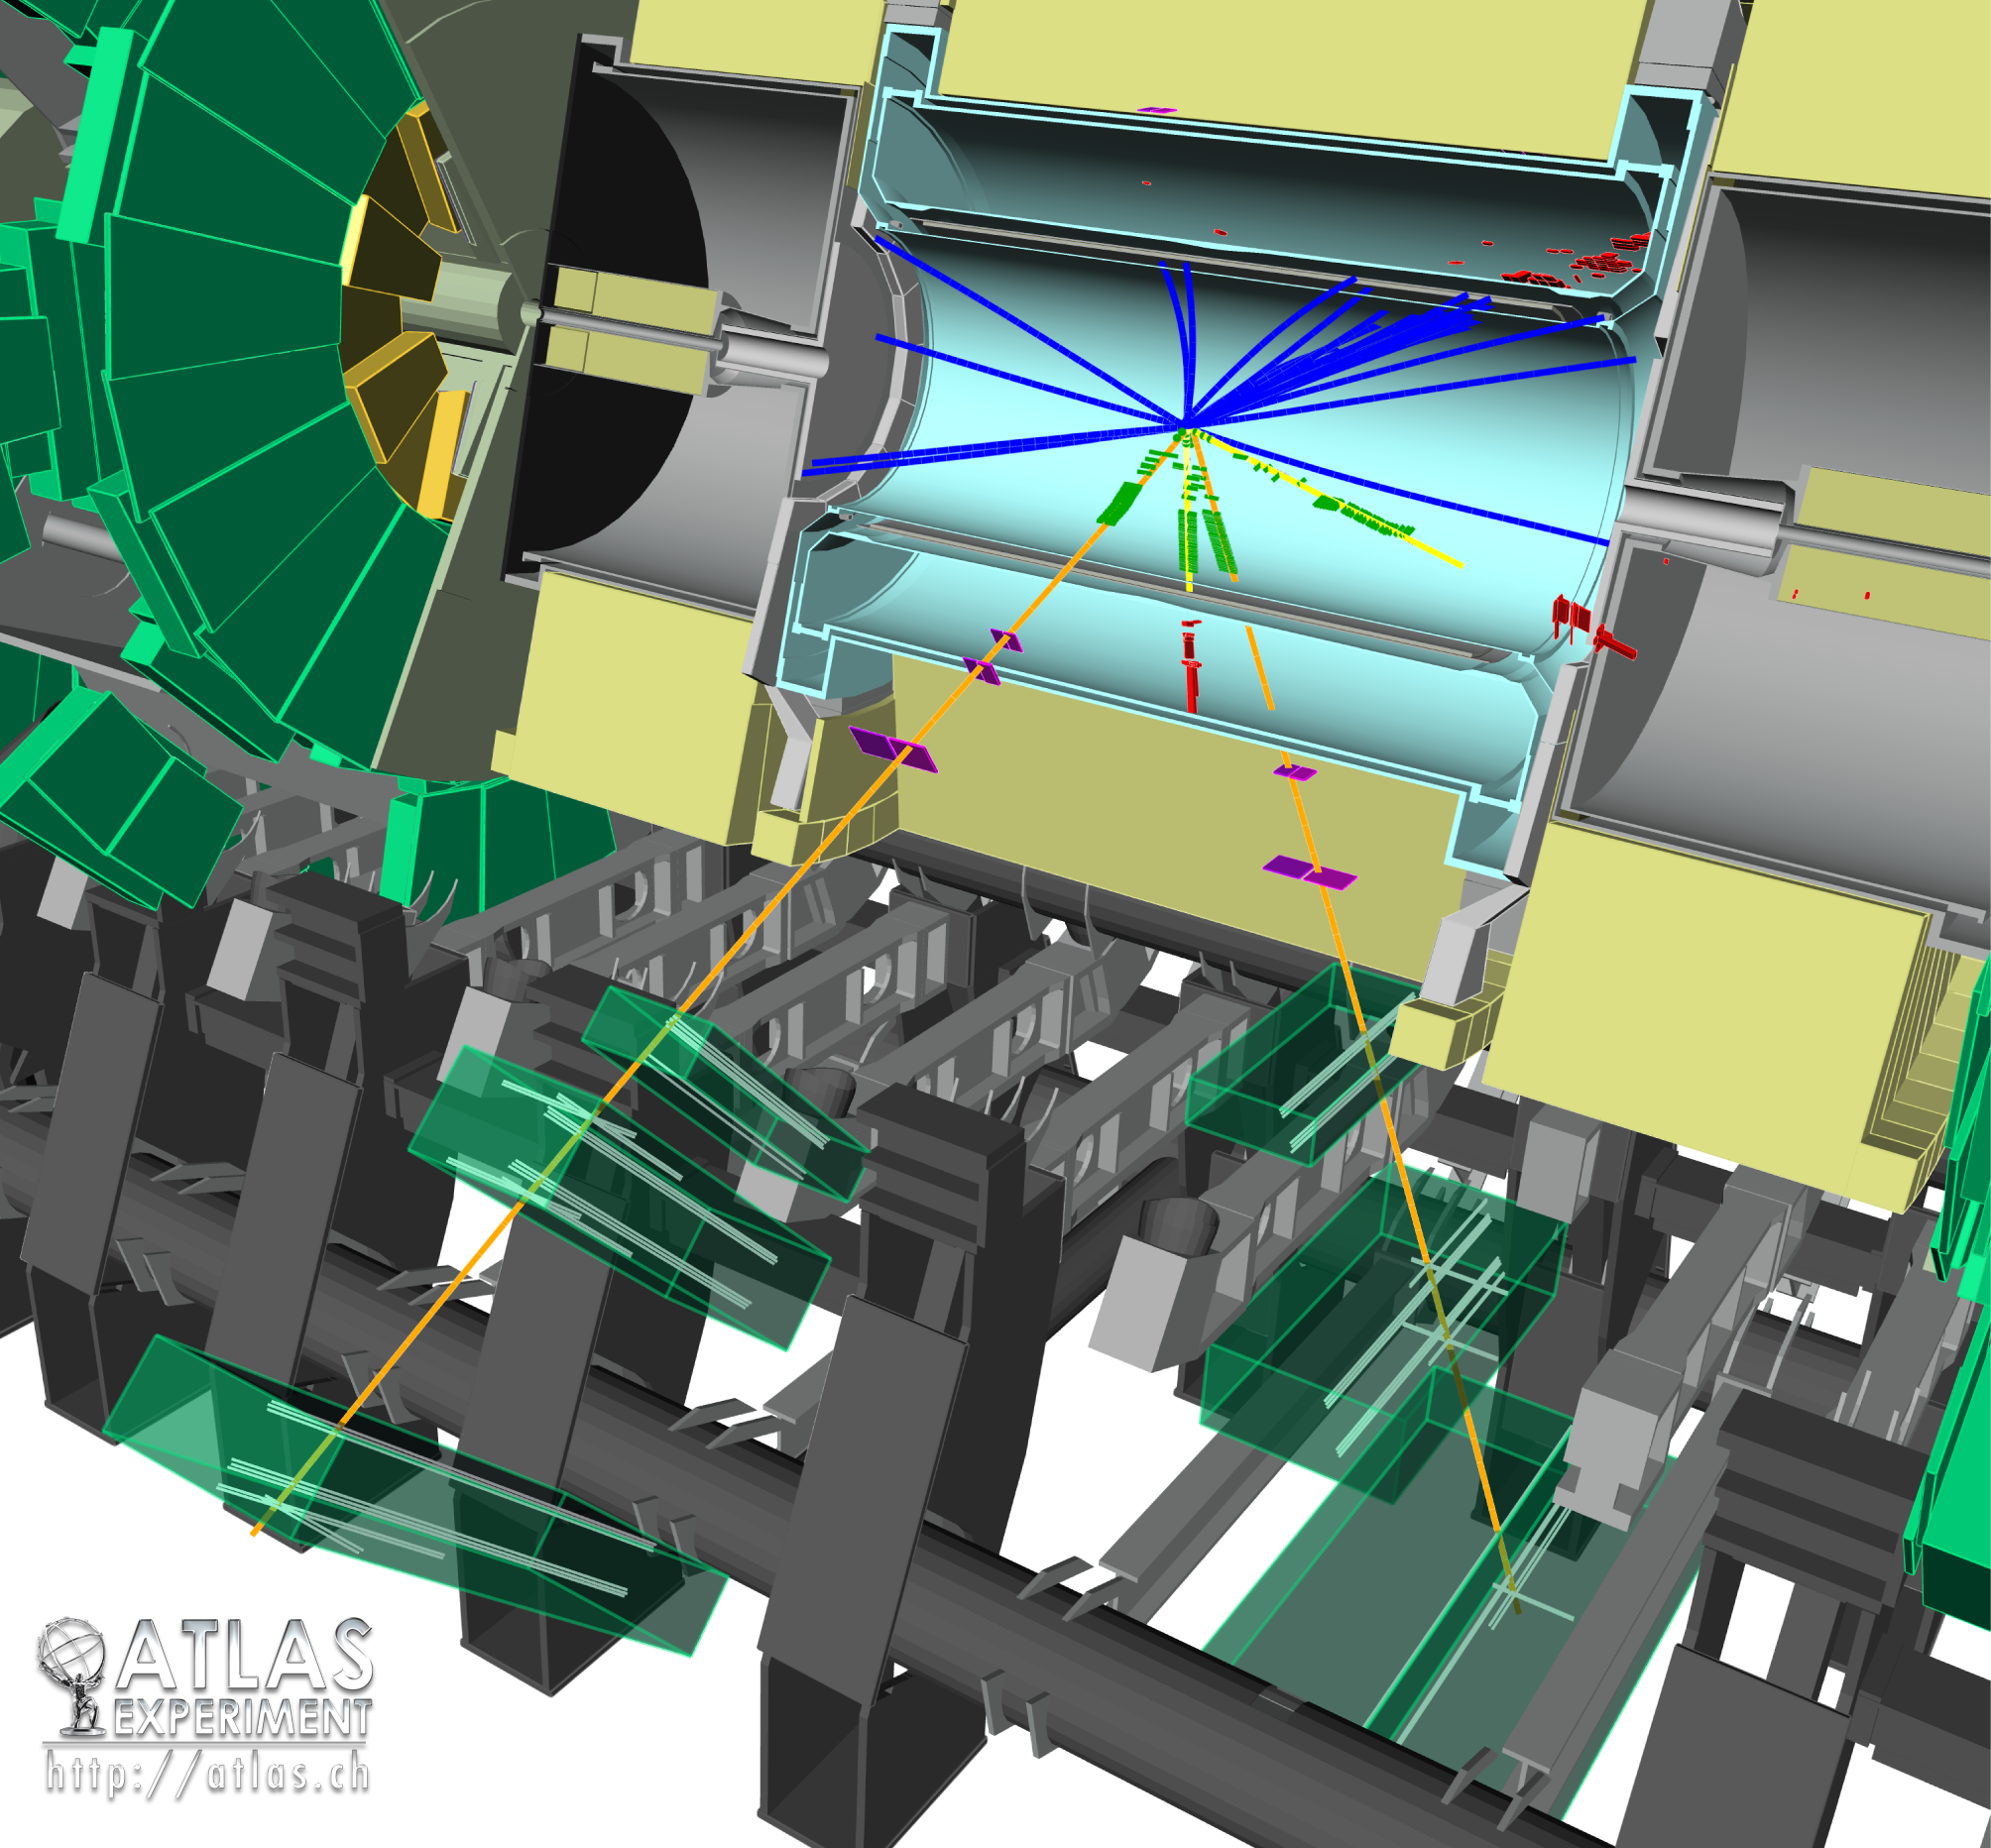
\includegraphics[width=0.8\textwidth]{montecarlo/figures/higgs_event_csc}}
	\caption{Display of a high-$p_T$ $H \to ZZ*\to ee\mu\mu$ decay ($m_H$ = 130~GeV), 
        after full simulation and reconstruction in the ATLAS detector. Picture from \url{http://www.atlas.ch}. \label{fig:atlasdisplay}}
\end{center}\end{figure}


The detector simulation relies on the usage of two databases: the 
{\it geometry database} contains the information on the detector volumes
like dimensions, geometry, position and material composition, while
the {\it conditions database} is constantly updated with the information
on the real detector real-time conditions as dead channels, misalignments,
temperature. Since conditions vary from run to run, it is important that
the detector simulation reproduces as close as possible the real status
of ATLAS during a particular data period. Also for this reason, Monte
Carlo samples are regularly reproduced consistently with {\it data reprocessings}
or {\it data releases}.  For the analyses presented in this dissertation,
the Monte Carlo production tagged as \texttt{mc12} is used, performed
within release 17 of the ATLAS analysis framework \texttt{ATHENA}~\cite{Calafiura:2005zz}.



\section{Monte Carlo samples corrections}\label{sec:mcweights}

At the end of the full Monte Carlo simulation chain, after the detector simulation
and event reconstruction steps, the generated samples need some corrections to
better model data. The main event reweighting is to correct Monte Carlo samples to
the correct theoretical cross section of the process and to the number of expected
data events, which comes from the luminosity measurements. As typical in Monte
Carlo techniques, an higher number of randomly produced events assures a better modeling
of the system under study, and therefore usually a very high number of events are
produced for each sample to maximize the confidence that all the relevant configurations
have been copiously simulated. The event weight $w$ to be applied (event by event) is defined
as:
\begin{equation}\label{eq:mcweight}
w = \dfrac{\sigma\times k}{N}\int \mathcal L dt,
\end{equation}
where $\sigma$ is the process theoretical cross section, $N$ is the number of Monte
Carlo events, $\int \mathcal L dt$ the integrated luminosity and $k$ is the so-called
$k-$factor, which is a correction to higher orders as, e.g., to bring the accuracy
of a LO cross section computation to the NLO.

Furthermore, a weight to account for pile-up effect is to be applied, to match the
expected number of interactions per bunch crossing $<\mu>$ in real data-taking conditions. 
